\usepackage{amsmath, amsthm, amssymb, amsfonts}
\usepackage{thmtools}
\usepackage{graphicx}
\usepackage{setspace}
\usepackage{geometry}
\usepackage{float}
\usepackage{hyperref}
\usepackage[utf8]{inputenc}
\usepackage[english]{babel}
\usepackage{framed}
\usepackage[dvipsnames]{xcolor}
\usepackage{tcolorbox}

\colorlet{LightGray}{White!90!Periwinkle}
\colorlet{LightOrange}{Orange!15}
\colorlet{LightGreen}{Green!15}

\newcommand{\HRule}[1]{\rule{\linewidth}{#1}}

\declaretheoremstyle[name=Theorem,]{thmsty}
\declaretheorem[style=thmsty,numberwithin=section]{theorem}
\tcolorboxenvironment{theorem}{colback=LightGray}

\declaretheoremstyle[name=Proposition,]{prosty}
\declaretheorem[style=prosty,numberlike=theorem]{proposition}
\tcolorboxenvironment{proposition}{colback=LightOrange}

\declaretheoremstyle[name=Principle,]{prcpsty}
\declaretheorem[style=prcpsty,numberlike=theorem]{principle}
\tcolorboxenvironment{principle}{colback=LightGreen}

\setstretch{1.2}
\geometry{
    textheight=9in,
    textwidth=5.5in,
    top=1in,
    headheight=12pt,
    headsep=25pt,
    footskip=30pt
}

% ------------------------------------------------------------------------------


% ------------------------------------------------------------------------------
% Cover Page and ToC
% ------------------------------------------------------------------------------

\title{ \normalsize \textsc{}
		\\ [2.0cm]
		\HRule{1.5pt} \\
		\LARGE \textbf{\uppercase{Git Assignment}
		\HRule{2.0pt} \\ [0.6cm] \LARGE{} \vspace*{10\baselineskip}}
		}
\date{}
\author{\textbf{Mahsa Rahimian} \\ 
		Mashsa Rahimian \\
		University of Colorado/Colorado Springs\\
		09/27/2023}

\maketitle
\newpage


% ------------------------------------------------------------------------------

\section{Git assignment}

\begin{text}
In this , I will copy some of my first assignments about myself, including photos. 
My goal of taking this course is to equip myself with the knowledge and tools essential for the successful realization of my upcoming research which is about software defined networking (SDN) and integrating this topic with Path-Aware Risk Scores for Access Control. Integrating these two topics could make access controls way more secure by considering not just who's trying to access something, but also the path they're taking and the situation around it.
This is my first semester at the University of Colorado, Colorado Springs (UCCS), and I'm eager to start working on this exciting topic. What I'm hoping to get out of this course is a bunch of tools and knowledge to supercharge my research skills. I want to learn all about different ways to do research, improve how I read and understand things, and get better at writing my ideas down.
Just to give you a little background, I've been on a bit of an academic journey already. I spent two years as a Ph.D. student at the University of Colorado Denver, and before that, I got my master's degree in Information Technology from Colorado Technical University.
I'm thrilled to be here, eager to learn, and really looking forward to using what I
learn to make a real impact in the world of computer science. 
I utilized Google Scholar as a valuable tool for locating research papers pertinent to my area of interest. For effective management of bibliographic data and associated research materials like PDF files, I tried to use Zotero to be an invaluable reference management tool. To enhance my remote research capabilities, I set up the UCCS VPN, granting me access to UCCS resources even when working off-campus.
\begin{figure}
    \center
    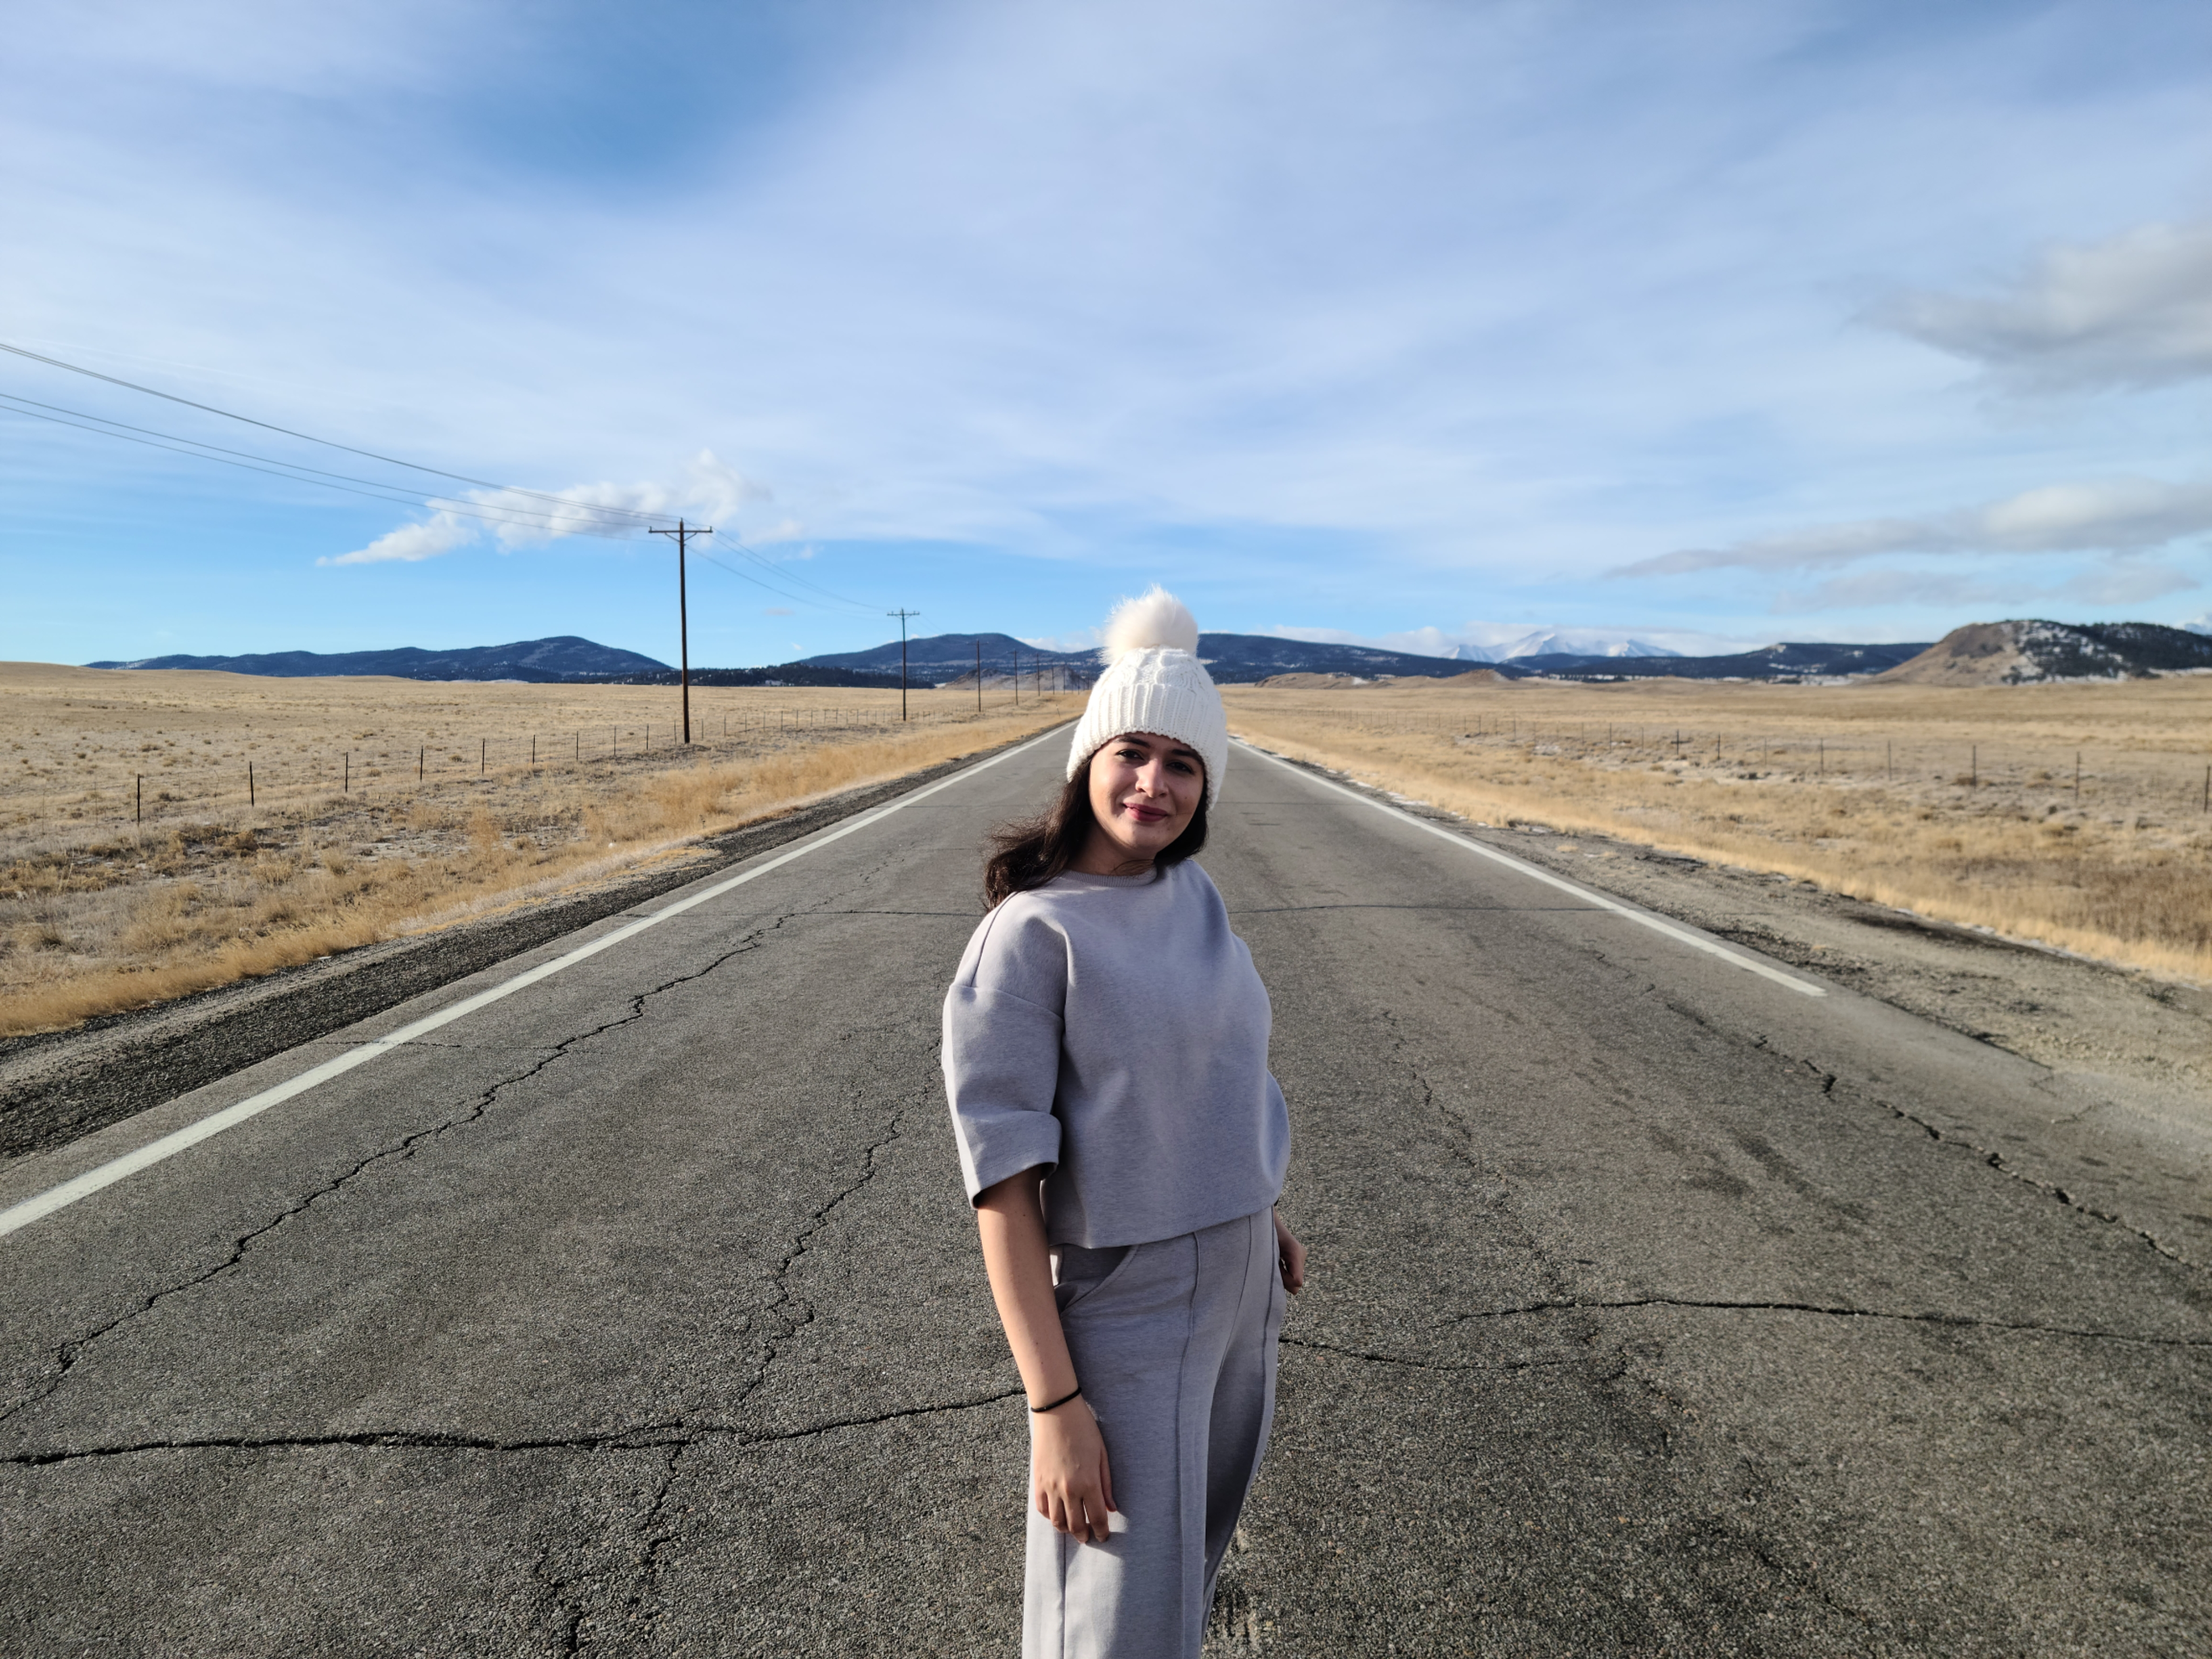
\includegraphics[scale=0.06]{Rahimian-F23/Figures/picture 1.jpg}
    \caption{Photo of myself}
\end{figure}

\section{Tools/ My research interest}
\begin{text}
In the initial stages of using Google Scholar, I encountered a challenge in refining my search results to precisely match my research criteria. However, I overcame this hurdle by employing the advanced search features, which significantly improved the relevance of the retrieved papers.
Navigating LaTeX proved to be another obstacle, particularly since I had not used it extensively for some time. Yet, through the aid of YouTube tutorials, I managed to regain my familiarity with LaTeX, enabling me to confidently resume working with it.
Through these tools and strategies, I have taken significant strides in streamlining my research process, from efficient paper discovery to effective reference management. Overcoming challenges has only served to enhance my adaptability and proficiency in my academic pursuits.
I would like to describe the three most related papers to my research. First, I would like to start with a paper titled Path-Aware Risk Scores for Access Control in
Zero-Trust Architectures 
\cite{seaton2022poster}. In summary, the paper introduces a context-sensitive technique that enhances access control in zero-trust architectures by assigning risk scores to paths taken by access requests. This approach addresses the need for fine-grained monitoring and enforcement and demonstrates improved path selection compared to traditional routing algorithms.
another paper that was intersting to me was Sidecar-based Path-aware Security for Microservices \cite{meadows2023sidecar}. the paper introduces a novel approach to improve the security of microservice architectures. The proposed infrastructure focuses on path-based anomaly detection and access control without the need for modifying existing software. By deploying trusted proxies and using signed tokens for path validation, the approach reduces the attack surface and enhances the security and resiliency of microservice-based applications that handle sensitive data.
and the third paper that I would like to describe it breifly is EPIC: Every Packet Is Checked in the Data Plane of a Path-Aware Internet \cite{legner2020epic}. The paper focuses on path-aware networking, a new network architecture that offers solutions to security issues in today's Internet while improving efficiency and giving end users control over data paths. The authors highlight three important issues: the need for network operators to apply their own rules for efficient path selection, the ability of end users to verify data forwarding, and the authentication of packet sources by intermediate routers and recipients. 
\end{text}

\



% ------------------------------------------------------------------------------
% Reference and Cited Works
% ------------------------------------------------------------------------------

\bibliographystyle{IEEEtran}
\bibliography{References.bib}

% ------------------------------------------------------------------------------

\section{Questions}
\subsection{Question 1}
\paragraph{}
\subsection{Question 2}
\paragraph{}